\chapter{Założenia projektowe}
% DONE?: Zamieszczono analizę wymagań, funkcjonalnych i niefunkcjonalnych, razem z wizualizacją funkcji za pomocą makiet \\\  zwykle projekty informatyczne zaczynają się od studium wykonalności (i analizy dziedzinowej).
%        Potem pojawia się analiza wymagań, której wynikiem jest zestaw zachowań, jakimi powinna
%        charakteryzować się powstająca aplikacja z punktu widzenia użytkownika.
%        W efekcie po tym etapie powinno być wiadome, jakie aplikacja będzie oferować funkcje i do czego ma służyć.
%       U Pana etap analizy wymagań nie został wyraźnie zaznaczony. 
%       Analizę wymagań formalizuje się, stosując listy wyliczeniowe, diagramy przypadków użycia itp.
%       Temu wszystkiemu towarzyszyć mogą makiety interfejsu użytkownika.
%       Makiety służą bowiem jako język, którym projektant komunikuje się z użytkownikiem.
%       Są one też językiem komunikacji między projektantem a programistą
%       Ogólnie - tworzenie makiet można zaliczyć do etapu analizy wymagań funkcjonalnych
%       (makiety eksponują funkcje, które są wystawiane na graficznym interfejsie użytkownika)
W niniejszym rozdziale opisano szczegóły działań, jakie podjęto po analizie dziedzinowej. W~ich ramach zdefiniowano wymagania funkcjonalnych i niefunkcjonalnych dla budowanej aplikacji. Na tej bazie przystąpiono do zaprojektowania makiet interfejsu użytkownika. Następnie zdecydowano się na wybór wzorca projektowego, na podstawie którego miała się odbywać implementacja komponentów wchodzących w skład poszczególnych scen. Po zadeklarowaniu potrzebnych elementów przystąpiono do tworzenia grafik tych komponentów, w tym: grafiki przycisków, tekstu, grafik akordów. Następnie zajęto się implementacją widoków i funkcji. 

\section{Analiza wymagań}
\subsection{Wymagania funkcjonalne}
Docelowa aplikacja powinna oferować funkcje opisane poniżej.
\begin{itemize}
\item \textbf{Stroik gitarowy} -- ta funkcja powinna umożliwiać dostrojenie strun gitary. Zawierać on ma opcję wyboru nuty, do której struna ma docelowo zostać nastrojona. Stroik zawierać ma graficzną reprezentację aktualnego poziomu nastrojenia instrumentu, poprzez wyświetlanie na ekranie informacji, czy struna jest: niedostrojona, nastrojona, przestrojona.
\item \textbf{Metronom} -- ma umożliwiać przeprowadzenie treningu rytmu, pozwalająć na parametryzację wartości: bpm, taktu, metrum.
\item \textbf{Księga akordów} -- ma dostarczać informacje o aktualnie wyświetlanym akordzie i jego wariacji. Zawierać ona ma również przycisk zezwalający na zapis aktualnie wyświetlanego akordu, z możliwością zapisu do 3 akordów, które następnie dostępne będą w osobnym widoku. Osobny widok zawierać ma również diagram akordów.
\item \textbf{Koło kwintowe} -- ma się pojawiać z aktywnymi przyciskami, których naciśnięcie skutkować ma podświetleniem skali molowej, wraz z siedmioma akordami, które wpasowują się pod wybraną nutę.
\item \textbf{Trening słuchu} -- istotą tej funkcji ma być możliwość odgadywania odegranej nuty poprzez jej zagranie i zweryfikowanie poprawności udzielonej odpowiedzi. 
\end{itemize}

\subsection{Wymagania niefunkcjonalne}

Dla projektu ustalono wymagania niefunkcjonalne. Zebrano je w punktach poniżej.
\begin{itemize}
\item \textbf{Intuicyjny interfejs} -- aplikacja ma oferować prosty i przejrzysty interfejs, z możliwością włączenia pomocy kontekstowej wyjaśniająca działanie poszczególnych elementów w widoku.
\item \textbf{Kompatybilność z systemem Windows 10} --  aplikacja zostanie stworzona głównie dla urządzeń desktopowych, działających pod kontrolą systemu operacyjnego Windows 10 (i wyżej).
\item \textbf{Responsywność} -- czas odpowiedzi aplikacji nie powinien wynosić więcej niż 2 sekundy. 
\end{itemize}
% DONE?: Wyjaśnienie zamieszczone w podrozdziale "przebieg" \\\ proszę dodać wyjaśnienie, jaką ścieżką Pan poszedł rozpoczynając projekt.
%        z tego, co widzę, całą analizę wymagań załatwił Pan makietami. 
%        W sumie można tak zrobić. Proszę to jednak uzasadnić, by czytelnik nie miał wątpliwości, 
%        że to celowy zabieg, a nie przeoczenie !!! 


% DONE?: proszę przeredagować rozdział. W tej chwili wygląda on słabo - nie widać jakiejś myśli przewodniej.

% DONE: proszę uważać ze stosowaniem określenia "architektura aplikacji"
%        zwykle gdy pada to określenie to odnosi się ono do sposobu "poukładania" komponentów aplikacji w jakieś hierarchie czy warstwy, z wydzieleniem odpowiedzialności, określeniem mechanizmów przepływu informacji itd. U Pana zaś mamy termin ten pada w kontekście użycia wzorca projektowego MVC.

\section{Makiety}
Na rysunku~\ref{fig:makiety} przedstawiono zaprojektowane makiety interfejsu użytkownika. Makiety te mają przybliżyć ogólny zarys planowanego układu udostępnianych widoków wraz z rozmieszczeniem na nich funkcji. Końcowa wersja interfejsu użytkownika może od odbiegać od tej propozycji.
\begin{figure}[htb]
    \centering
		\begin{tabular}{ll}
		a) & b \\
		\vtop{\vskip-2ex\hbox{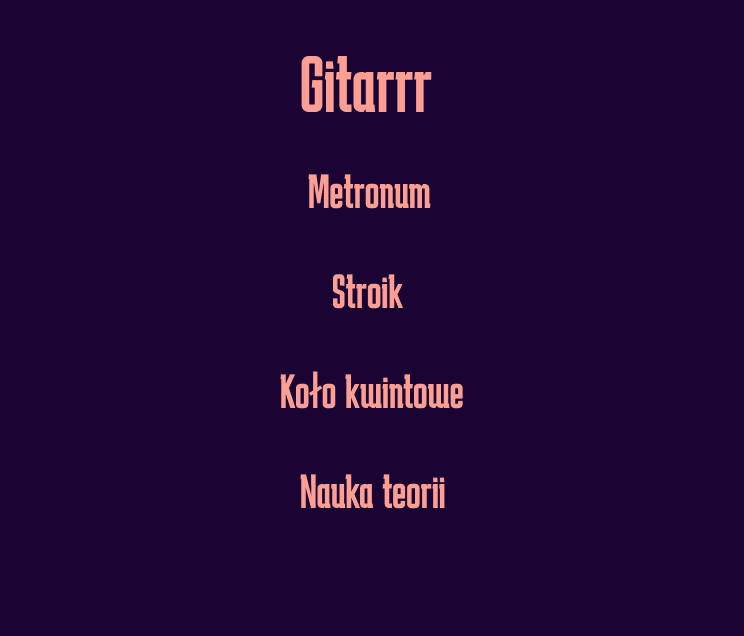
\includegraphics[width=0.4\linewidth]{rys03/MakMain}}} &
		\vtop{\vskip-2ex\hbox{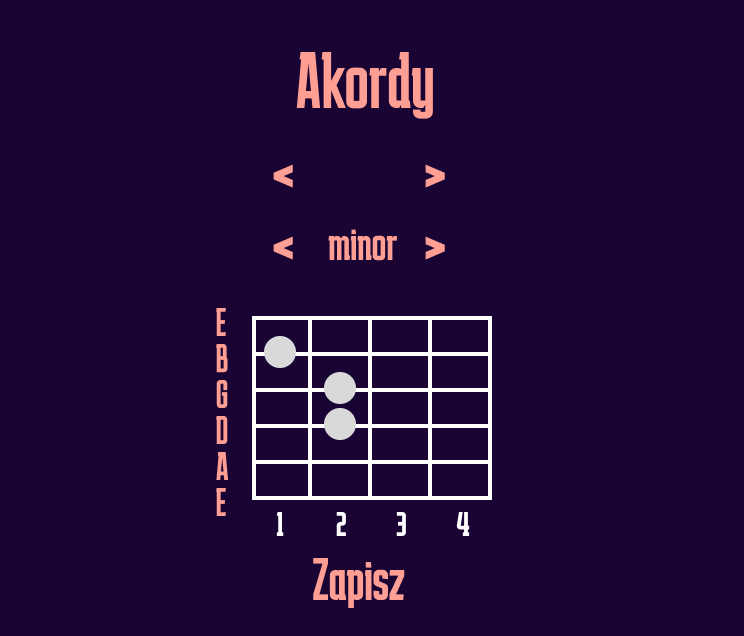
\includegraphics[width=0.4\linewidth]{rys03/MakAkordy}}} \\
		c) & d) \\
		\vtop{\vskip-2ex\hbox{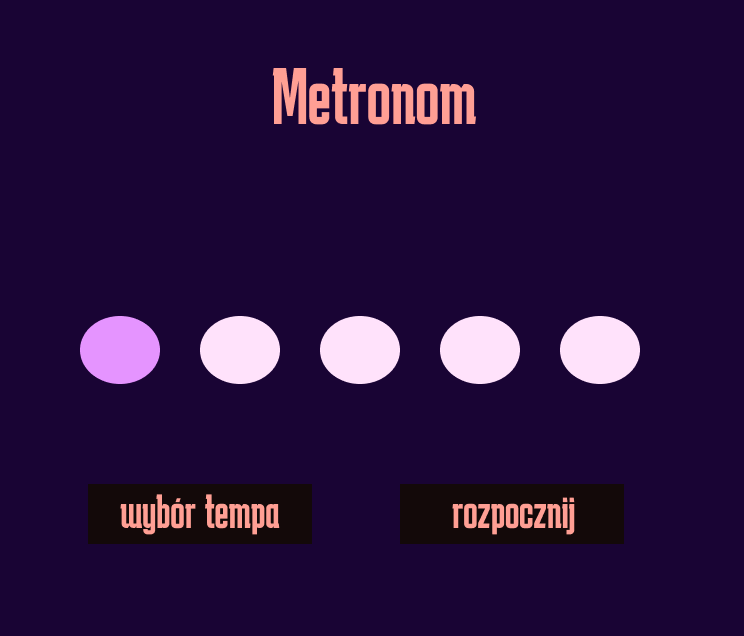
\includegraphics[width=0.4\linewidth]{rys03/MakMetronom}}} &
		\vtop{\vskip-2ex\hbox{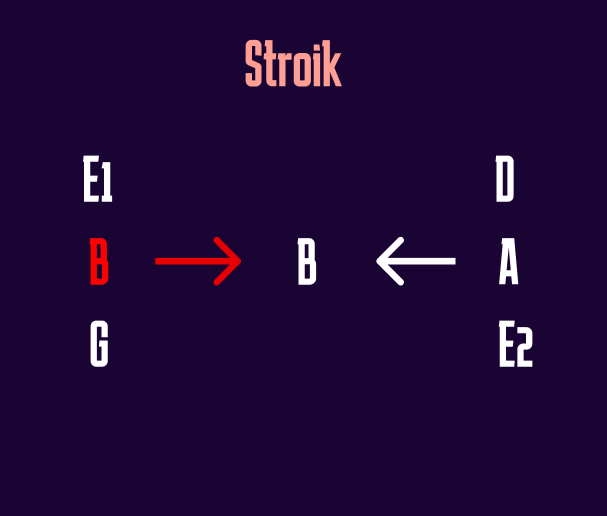
\includegraphics[width=0.4\linewidth]{rys03/MakStroik}}} \\
		e) & f) \\
		\vtop{\vskip-2ex\hbox{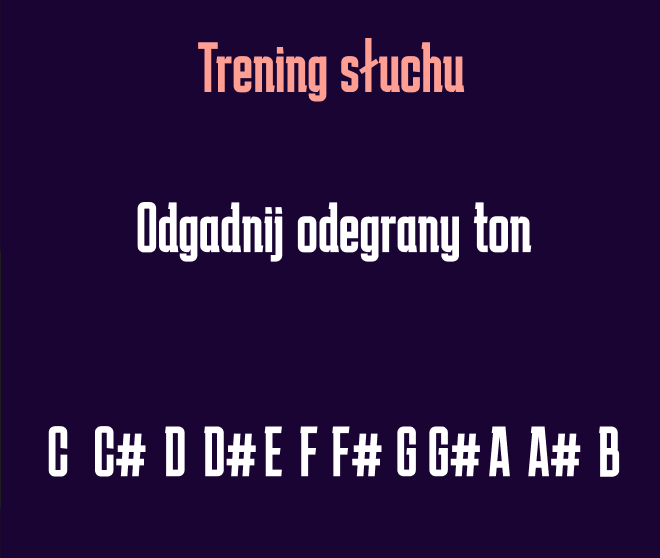
\includegraphics[width=0.4\linewidth]{rys03/MakTrening}}} &
		\vtop{\vskip-2ex\hbox{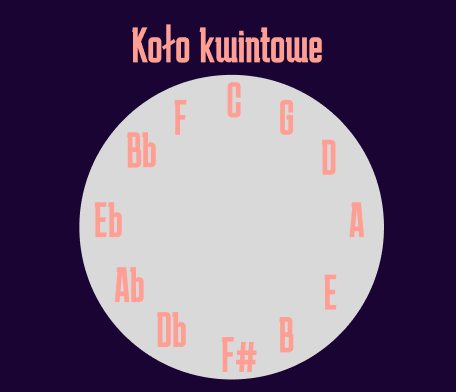
\includegraphics[width=0.4\linewidth]{rys03/MakKK}}}	
		\end{tabular}
        \caption{Zaprojektowane makiety interfejsu: a) scena główna, b) księga akordów, c) metronom, d) stroik, e) trening słuchu, f) koło kwintowe}
        \label{fig:makiety}
\end{figure}


\section{Projekt aplikacji}
% DONE: proszę zadbać o to, by na końcach linii nie pozostały samotne literki
Projekt aplikacji stworzono w sposób taki, aby każda z poszczególnych funkcji była przejrzysta, a sama aplikacja umożliwiała płynne przełączanie pomiędzy widokami. Zastosowano wzorzec \emph{Model-View-ViewModel}, umożliwiający rozdzielenie logiki aplikacji, interfejsu oraz zarządzania danymi. W skład wzorca wchodzą poniższe 3 elementy:

\begin{itemize}
	\item \emph{Model}: Logika danych aplikacji, zawierająca dane akordów, dźwięków, tempo metronomu,
	\item \emph{View}: Zawiera sceny samej aplikacji, dla każdej funkcji zaplanowano osobny widok (sceny),
	\item \emph{ViewModel}: Do każdej ze scen przypisany został kontroler odpowiedniej sceny umożliwiający komunikację pomiędzy widokiem, a modelem, zawiera on logikę aplikacji, oraz definicje funkcji potrzebnych w danej scenie.
\end{itemize}

\subsection{Projekt poszczególnych scen}
Poniżej omówiono schemat każdej z projektowanych scen aplikacji, zaznaczając komponenty wchodzące w skład danego narzędzia, wyjaśniając co jest ich celem oraz jakie technologie wykorzystano w ich implementacji. 

\subsubsection{Scena 1: Scena Główna}

\begin{itemize}

\item Cel: Reprezentacja możliwości wyboru, oraz udzielenie użytkownikowi dostępu do poszczególnych narzędzi za pomocą czytelnych przycisków, które po naciśnięciu przechodzą do odpowiadającej im sceny z danym narzędziem. 
\item Komponenty: Elementami wchodzącymi w skład sceny głównej są przyciski (jest ich 5): stroik, metronom, koło kwintowe, księga akordów, trening słuchu. Dodatkowo scena główna zawiera obiekt tekstowy z logiem aplikacji.  
\item Technologie: Do realizacji tej oto sceny użyto wbudowaną bibliotekę w silnik Unity, a mianowicie Unity.UI, umożliwiającą utworzenie graficznego interfejsu uzytkownika. 
\item Komunikacja: Każdy z przycisków wchodzących w skład sceny podłączony jest pod kontroler sceny, służący jako pośrednik, w skrypcie należącym do kontrolera poszczególnym przyciskom przypisywana jest funkcja odpowiadająca za załadowanie odpowiedniej sceny. 
\end{itemize}

\subsubsection{Scena 2: Stroik}

\begin{itemize}
\item Cel: Udostępnienie możliwości nastrojenia gitary poprzez wybór docelowej struny, do której użytkownik chce nastroić instrument. Następnie zagrane przez użytkownika dźwięki analizowane będą, a wyniki analizy reprezentowane zostaną jako informacja odnośnie tego, czy ton należy obniżyć czy podwyższyć.
\item Komponenty: W skład sceny wchodzi mikrofon, analizator dźwięku, przyciski odpowiadające strunom na gitarze, oraz indykator aktualnego poziomu nastrojenia instrumentu.  
\item Technologie: Do użytych technologii wykorzystano bibliotekę opartą na otwartej licencji służącą do analizy dostarczanego dźwięku \cite{AudioPitchEstimator}, oraz wyciągnięcie z niego częstotliwości zagranej nuty. Dodatkowo do stworzenia graficznego interfejsu posłużono się biblioteką Unity.UI.   
\item Komunikacja: Użyto kontroler sceny, aby umożliwić komunikacje pomiędzy elementami graficznymi a analizatorem dźwięku. 
\end{itemize}

\subsubsection{Scena 3: Metronom}

\begin{itemize}
\item Cel: Zapewnienie użytkownikowi możliwości treningu rytmu podczas gry, poprzez reprezentację poszczególnych taktów zsynchronizowanych z dźwiękiem "bitu".
\item Komponenty: Do realizacji tej sceny zastosowano przyciski umożliwiające parametryzację taktu, oraz bpm(ang. beats per minute). Wizualizacja metronomu odbywa się za pośrednictwem pojawiających się na ekranie kwadratów reprezentujących poszczególny takt, które zmieniają swoje kolory z białego na czarny, wraz z czasem wybijania danego rytmu.
\item Technologie: Skrypt napisany w języku C\# realizujący logikę działania metronomu.
\item Komunikacja: Poszczególne komponenty komunikują się ze sobą za pośrednictwem kontrolera sceny metronomu, zawierający odwołania do poszczególnych komponentów.
\end{itemize}

\subsubsection{Scena 4: Księga akordów}

\begin{itemize}
\item Cel: Wizualizacja pozycji akordów na gryfie, dla każdej nut, wraz z możliwymi wariancjami akordów.
\item Komponenty: Do komponentów należą przyciski odpowiadające za przeglądanie listy dostępnych akordów, element graficzny wizualizujący aktualnie wybrany akord, wraz z przyciskami odpowiadającymi za przełączenie sceny do widoku diagramu wszystkich możliwych akordów.
\item Technologie: Wbudowana biblioteka do obsługi graficznego interfejsu użytkownika - Unity.UI.
\item Komunikacja: Komponenty komunikują się ze sobą za pomocą menadżera sceny, przechowującego za pomoca listy graficzne reprezentacje akordów, które wyświetlane są w odpowiednich momentach. 
\end{itemize}

\subsubsection{Scena 5: Trening słuchu}

\begin{itemize}
\item Cel: Umożliwienie użytkownikowi przeprowadzenie ćwiczeń mających na celu nabycia umiejętności rozpoznawania granej nuty za pomocą samego słuchu.
\item Komponenty: Przyciski odpowiadające za wybór skali treningowej, przyciski odpowiadające za odpowiedź, po naciśnięciu których weryfikowana jest poprawność udzielonej odpowiedzi. Scena zawiera również system audio odpowiadający za odegranie dźwięku.
\item Technologie: Za odgrywanie dźwięków odpowiada biblioteka Unity.Sound, wraz z gotowym komponentem audio wbudowanym w silnik Unity.
\item Komunikacja: Za komunikację pomiędzy komponentami odpowiada menadzer sceny, łączący ze sobą przyciski, zawierający logike odpowiedzialną za działanie sceny.
\end{itemize}

\subsubsection{Scena 6: Koło kwintowe}

\begin{itemize}
	\item Cel: Wizualizacja koła kwintowego, wraz z skalą molową i durową.
	\item Komponenty: Elementy graficzne, w postaci przycisków, zawierające komponent image, który zawiera odpowiadającą nutę.
	\item Technologie: Użyto biblioteki Unity.UI do reprezentacji poszczególnych nut.
	\item Komunikacja: Komunikacja odbywa się poprzez menadżer sceny, zawierający logikę odpowiadającą za podświetlenie odpowiadających nut po naciśnięciu jednego z przycisków na kole kwintowym.
\end{itemize}

\subsubsection{Scena 7: Diagram akordów}

\begin{itemize}
	\item Cel: Wizualizacja wszystkich dostępnych akordów w aplikacji.
	\item Komponenty: Elementy graficzne, w postaci przycisków, zawierające komponent image, który zawiera odpowiadający akord.
	\item Technologie: Użyto biblioteki Unity.UI do reprezentacji poszczególnych nut.
	\item Komunikacja: Komunikacja odbywa się poprzez menadżer sceny, zawierający logikę odpowiadającą za uruchomienie widoku księgi akordów z wyświetlonym wybranym akordem.
\end{itemize}

\subsubsection{Scena 8: Zapisane akordy}

\begin{itemize}
	\item Cel: Wizualizacja zapisanych przez użytkownika akordów w scenie księgi akordów.
	\item Komponenty: Elementy graficzne zawierające komponent image, który zawiera odpowiadający akord.
	\item Technologie: Użyto biblioteki Unity.UI do reprezentacji poszczególnych akordów.
	\item Komunikacja: Komunikacja odbywa się poprzez menadżer sceny, zawierający logikę odpowiadającą komunikację ze sceną księgi akordów i przekazaniu zapisanych akordów.
\end{itemize}